\begin{enumerate}
\def\labelenumi{\arabic{enumi}.}
\setcounter{enumi}{1}
\item
  \textbf{System Architecture and Concept of Operations}
\end{enumerate}

\subsection{System Architecture}

Helike \#213 is a PocketQube 1P (50$\times$50$\times$50~mm, $\sim$200~g)
whose central subsystem is the SRAB — the bioinspired autorotative
recovery system. The satellite is organized in five functional blocks:

\begin{center}
{\small
\setlength{\tabcolsep}{6pt}
\begin{tabularx}{\linewidth}{>{\raggedright}p{3cm}X}
\toprule
\textbf{Block} & \textbf{Components} \\
\midrule
Recovery (SRAB) & 2--4 autorotative wings, passive deployment \\
EPS & Li-Ion battery + BMS, RBF pin, 2 kill switches \\
Avionics & ESP32-C3 Super Mini, FSM + cooperative scheduler \\
Sensors & BME280 (pressure/temp/humidity), ICM-20602 (6-axis IMU) \\
Telemetry & LoRa RFM95W 915 MHz, GPS NEO-8M, SD + LittleFS \\
\bottomrule
\end{tabularx}
}
\end{center}

\begin{figure}[htbp]
\centering
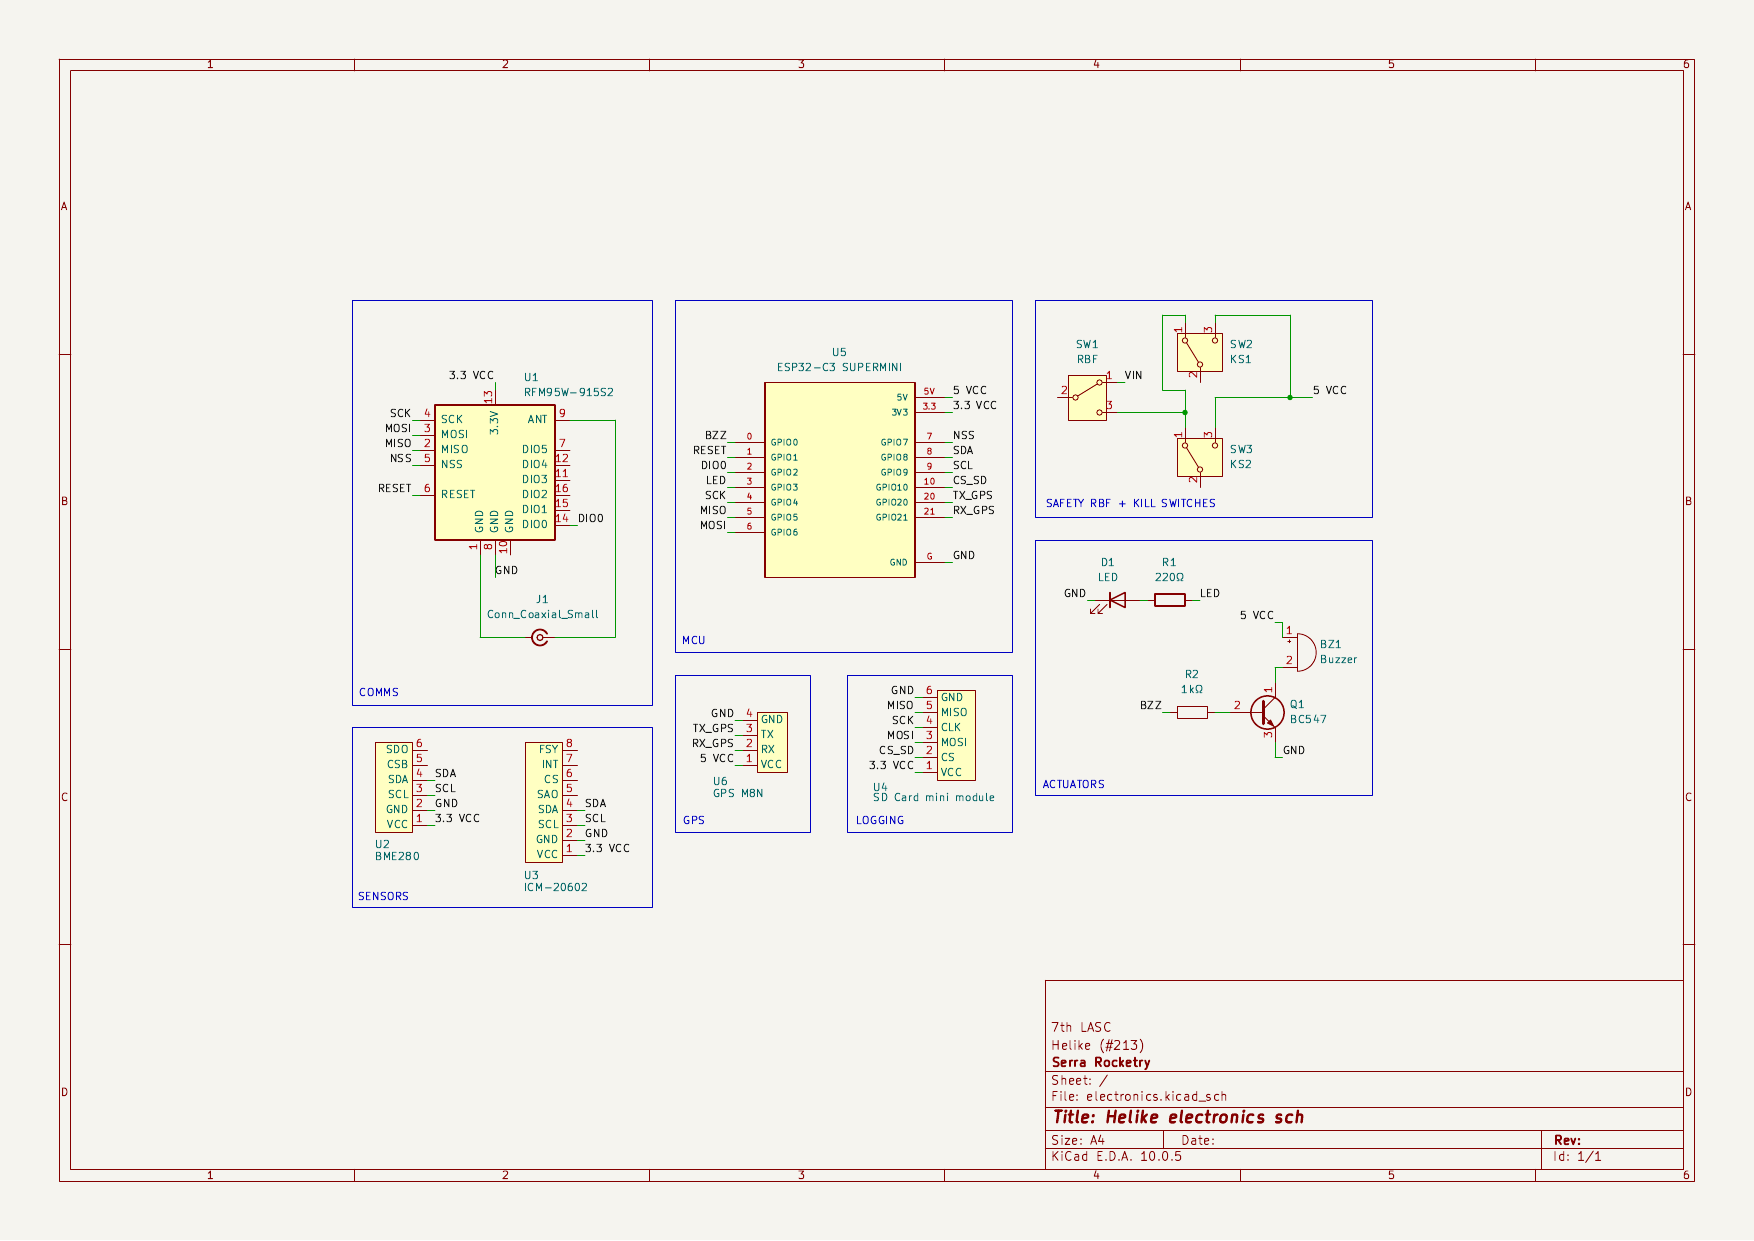
\includegraphics[width=0.85\textwidth]{figures/fig_schematic.png}
\caption{Electrical schematic of Helike \#213 (KiCad). U1: ESP32-C3
Super Mini; U2: LoRa RFM95W-915S2; U3: BME280; U4: ICM-20602; U5: GPS
NEO-8M; U6: SD card module; SW1/SW2: kill switches (Z axis); SW3: RBF
pin; J1: SMA antenna; D1/BZ1: status LED and buzzer.}
\label{fig:schematic}
\end{figure}

\subsection{Subsystem Descriptions}

\subsubsection{Recovery (SRAB)}

The SRAB is a passive recovery system composed of 4 autorotative wings
(stowed during flight, deployed by ejection) that convert the potential
energy of the fall into rotational kinetic energy, reducing terminal
velocity. It has:

\begin{itemize}
\item \textbf{No actuators:} no servo, no pyrotechnics, no deployment
  electronics.
\item \textbf{No software dependency:} recovery works even with total
  loss of the avionics.
\item \textbf{Predicted terminal velocity:} 10.05~m/s (Test 2, Asa2
  geometry), within the SCSM range.
\item \textbf{Geometric redundancy:} the wing count (4) provides
  inherent redundancy — loss of one wing degrades performance but does
  not prevent recovery.
\end{itemize}

\subsubsection{Electrical Power System}

\begin{itemize}
\item \textbf{Energy:} Li-Ion battery (6000~mAh) with BMS (overcharge,
  overdischarge, short-circuit, overcurrent protection).
\item \textbf{Autonomy:} $>$40~h (margin $>$10$\times$ over the SCSM
  $\geq$4~h requirement). Power budget $\sim$145~mA average.
\item \textbf{Safety:} 2 kill switches (SW1/SW2, SPDT, Z axis) +
  RBF pin (SW3) cutting all energy. The satellite only powers on at
  ejection (REC 10.1.1 independence from the rocket).
\end{itemize}

\subsubsection{Avionics and Telemetry}

\begin{itemize}
\item \textbf{MCU:} ESP32-C3 Super Mini (single-core RISC-V), FSM +
  cooperative scheduler.
\item \textbf{Sensors:} BME280 (pressure/temperature/humidity) +
  ICM-20602 (6-axis IMU: accelerometer + gyroscope) — used for flight
  phase detection and SRAB rotation analysis.
\item \textbf{Telemetry:} LoRa RFM95W 915~MHz (downlink of sensor
  telemetry) + GPS NEO-8M (post-landing position).
\item \textbf{Storage:} SD card with LittleFS fallback on internal
  flash.
\item \textbf{Location support:} 3 ground beacons measuring RSSI for
  triangulation after landing.
\end{itemize}

\subsection{Concept of Operations}

The satellite follows a 9-phase FSM, aligned with the physical flight
profile:

\begin{enumerate}
\item \textbf{SAFE} — powered off (kill switches/RBF inserted),
  inert during integration.
\item \textbf{PRE-FLIGHT} — powered on at ejection, sensors
  initialized, first GPS fix attempted.
\item \textbf{BOOST} — high acceleration detected (IMU $>$ 2~g),
  high-frequency logging.
\item \textbf{COAST} — low/negative acceleration, minimal vertical
  velocity, apogee approaching.
\item \textbf{APOGEE} — pressure plateau detected, SRAB release
  armed.
\item \textbf{EJECTION + SRAB} — satellite released, SRAB wings
  deploy passively (no actuator).
\item \textbf{DESCENT} — SRAB autorotation, telemetry of rotation rate
  and descent velocity; LRR (Launch Readiness Review) parameters
  monitored.
\item \textbf{IMPACT} — impact detected by IMU, buzzer activated, GPS
  position stored.
\item \textbf{POST-LANDING} — low-power beacon mode: periodic LoRa
  transmissions (RSSI) + GPS position for recovery.
\end{enumerate}

\begin{figure}[htbp]
\centering
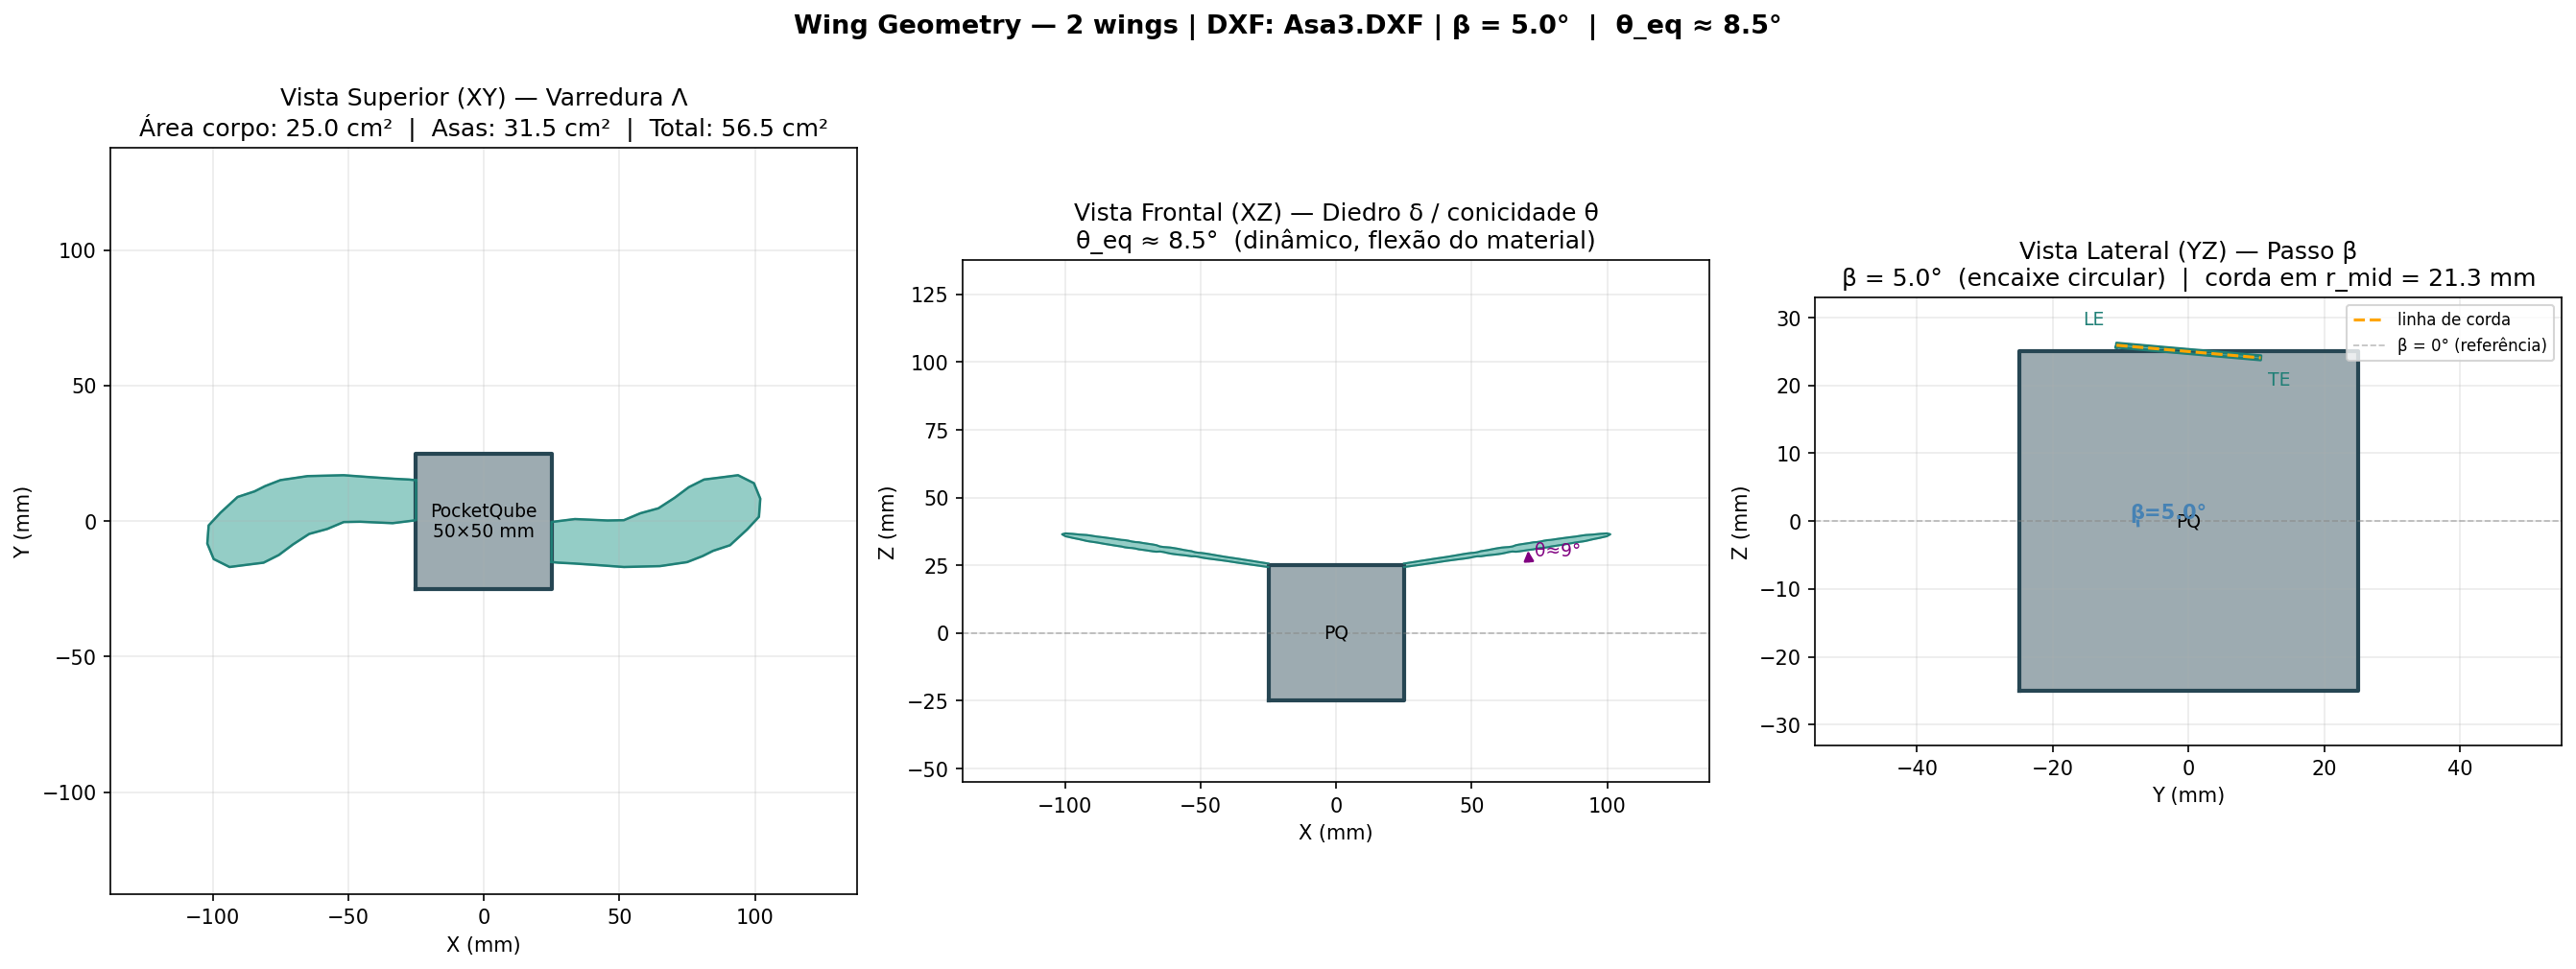
\includegraphics[width=0.9\textwidth]{figures/fig_asa3_geometry.png}
\caption{SRAB wing geometry views (Asa3): three orthogonal projections
of the wing + hub assembly used in the computational simulation and
drop tests.}
\label{fig:wing-geometry}
\end{figure}

% TODO: replace placeholder figure above with the final CAD renders /
% exploded view once available. fig_asa3_geometry.png is the
% computational geometry used in the SRAB model.
